
\documentclass[a4paper,11pt]{article}
\usepackage[a4paper, margin=8em]{geometry}

% usa i pacchetti per la scrittura in italiano
\usepackage[french,italian]{babel}
\usepackage[T1]{fontenc}
\usepackage[utf8]{inputenc}
\frenchspacing 

% usa i pacchetti per la formattazione matematica
\usepackage{amsmath, amssymb, amsthm, amsfonts}

% usa altri pacchetti
\usepackage{gensymb}
\usepackage{hyperref}
\usepackage{standalone}

\usepackage{colortbl}

\usepackage{xstring}
\usepackage{karnaugh-map}

% imposta il titolo
\title{Electronics for Embedded Systems notes}
\author{Luca Seggiani}
\date{2026}

% spaziatura liste
\usepackage{enumitem}
\setlist[itemize]{noitemsep, topsep=4pt, partopsep=0pt, parsep=2pt, leftmargin=*}
\setlist[enumerate]{noitemsep, topsep=4pt, partopsep=0pt, parsep=2pt, leftmargin=*}

% imposta lo stile
% usa helvetica
\usepackage[scaled]{helvet}
% usa palatino
\usepackage{palatino}
% usa un font monospazio guardabile
\usepackage{lmodern}

\renewcommand{\rmdefault}{ppl}
\renewcommand{\sfdefault}{phv}
\renewcommand{\ttdefault}{lmtt}

% circuiti
\usepackage{circuitikz}
\usetikzlibrary{babel}

% testo cerchiato
\newcommand*\circled[1]{\tikz[baseline=(char.base)]{
            \node[shape=circle,draw,inner sep=2pt] (char) {#1};}}

% disponi il titolo
\makeatletter
\renewcommand{\maketitle} {
	\begin{center} 
		\begin{minipage}[t]{.8\textwidth}
			\textsf{\huge\bfseries \@title} 
		\end{minipage}%
		\begin{minipage}[t]{.2\textwidth}
			\raggedleft \vspace{-1.65em}
			\textsf{\small \@author} \vfill
			\textsf{\small \@date}
		\end{minipage}
		\par
	\end{center}

	\thispagestyle{empty}
	\pagestyle{fancy}
}
\makeatother

% disponi teoremi
\usepackage{tcolorbox}
\newtcolorbox[auto counter, number within=section]{theorem}[2][]{%
	colback=blue!10, 
	colframe=blue!40!black, 
	sharp corners=northwest,
	fonttitle=\sffamily\bfseries, 
	title=Theorem~\thetcbcounter: #2, 
	#1
}

% disponi definizioni
\newtcolorbox[auto counter, number within=section]{definition}[2][]{%
	colback=red!10,
	colframe=red!40!black,
	sharp corners=northwest,
	fonttitle=\sffamily\bfseries,
	title=Definition~\thetcbcounter: #2,
	#1
}

% disponi codice
\usepackage{listings}
\usepackage[table]{xcolor}

\definecolor{codegreen}{rgb}{0,0.6,0}
\definecolor{codegray}{rgb}{0.5,0.5,0.5}
\definecolor{codepurple}{rgb}{0.58,0,0.82}
\definecolor{backcolour}{rgb}{0.95,0.95,0.92}

\lstdefinestyle{codestyle}{
		backgroundcolor=\color{black!5}, 
		commentstyle=\color{codegreen},
		keywordstyle=\bfseries\color{magenta},
		numberstyle=\sffamily\tiny\color{black!60},
		stringstyle=\color{green!50!black},
		basicstyle=\ttfamily\footnotesize,
		breakatwhitespace=false,         
		breaklines=true,                 
		captionpos=b,                    
		keepspaces=true,                 
		numbers=left,                    
		numbersep=5pt,                  
		showspaces=false,                
		showstringspaces=false,
		showtabs=false,                  
		tabsize=2
}

\lstdefinestyle{shellstyle}{
		backgroundcolor=\color{black!5}, 
		basicstyle=\ttfamily\footnotesize\color{black}, 
		commentstyle=\color{black}, 
		keywordstyle=\color{black},
		numberstyle=\color{black!5},
		stringstyle=\color{black}, 
		showspaces=false,
		showstringspaces=false, 
		showtabs=false, 
		tabsize=2, 
		numbers=none, 
		breaklines=true
}

\lstdefinelanguage{x86}{ 
  keywords={AAA, AAD, AAM, AAS, ADC, ADCB, ADCW, ADCL, ADD, ADDB, ADDW, ADDL, AND, ANDB, ANDW, ANDL,
        ARPL, BOUND, BSF, BSFL, BSFW, BSR, BSRL, BSRW, BSWAP, BT, BTC, BTCB, BTCW, BTCL, BTR, 
        BTRB, BTRW, BTRL, BTS, BTSB, BTSW, BTSL, CALL, CBW, CDQ, CLC, CLD, CLI, CLTS, CMC, CMP,
        CMPB, CMPW, CMPL, CMPS, CMPSB, CMPSD, CMPSW, CMPXCHG, CMPXCHGB, CMPXCHGW, CMPXCHGL,
        CMPXCHG8B, CPUID, CWDE, DAA, DAS, DEC, DECB, DECW, DECL, DIV, DIVB, DIVW, DIVL, ENTER,
        HLT, IDIV, IDIVB, IDIVW, IDIVL, IMUL, IMULB, IMULW, IMULL, IN, INB, INW, INL, INC, INCB,
        INCW, INCL, INS, INSB, INSD, INSW, INT, INT3, INTO, INVD, INVLPG, IRET, IRETD, JA, JAE,
        JB, JBE, JC, JCXZ, JE, JECXZ, JG, JGE, JL, JLE, JMP, JNA, JNAE, JNB, JNBE, JNC, JNE, JNG,
        JNGE, JNL, JNLE, JNO, JNP, JNS, JNZ, JO, JP, JPE, JPO, JS, JZ, LAHF, LAR, LCALL, LDS,
        LEA, LEAVE, LES, LFS, LGDT, LGS, LIDT, LMSW, LOCK, LODSB, LODSD, LODSW, LOOP, LOOPE,
        LOOPNE, LSL, LSS, LTR, MOV, MOVB, MOVW, MOVL, MOVSB, MOVSD, MOVSW, MOVSX, MOVSXB,
        MOVSXW, MOVSXL, MOVZX, MOVZXB, MOVZXW, MOVZXL, MUL, MULB, MULW, MULL, NEG, NEGB, NEGW,
        NEGL, NOP, NOT, NOTB, NOTW, NOTL, OR, ORB, ORW, ORL, OUT, OUTB, OUTW, OUTL, OUTSB, OUTSD,
        OUTSW, POP, POPL, POPW, POPB, POPA, POPAD, POPF, POPFD, PUSH, PUSHL, PUSHW, PUSHB, PUSHA, 
        RCLL, RCR, RCRB, RCRW, RCRL, RDMSR, RDPMC, RDTSC, REP, REPE, REPNE, RET, ROL, ROLB, ROLW,
        ROLL, ROR, RORB, RORW, RORL, SAHF, SAL, SALB, SALW, SALL, SAR, SARB, SARW, SARL, SBB,
        SBBB, SBBW, SBBL, SCASB, SCASD, SCASW, SETA, SETAE, SETB, SETBE, SETC, SETE, SETG, SETGE,
        SETL, SETLE, SETNA, SETNAE, SETNB, SETNBE, SETNC, SETNE, SETNG, SETNGE, SETNL, SETNLE,
        SETNO, SETNP, SETNS, SETNZ, SETO, SETP, SETPE, SETPO, SETS, SETZ, SGDT, SHL, SHLB, SHLW,
        SHLL, SHLD, SHR, SHRB, SHRW, SHRL, SHRD, SIDT, SLDT, SMSW, STC, STD, STI, STOSB, STOSD,
        STOSW, STR, SUB, SUBB, SUBW, SUBL, TEST, TESTB, TESTW, TESTL, VERR, VERW, WAIT, WBINVD,
        XADD, XADDB, XADDW, XADDL, XCHG, XCHGB, XCHGW, XCHGL, XLAT, XLATB, XOR, XORB, XORW, XORL},
  keywordstyle=\color{blue}\bfseries,
  ndkeywordstyle=\color{darkgray}\bfseries,
  identifierstyle=\color{black},
  sensitive=false,
  comment=[l]{\#},
  morecomment=[s]{/*}{*/},
  commentstyle=\color{purple}\ttfamily,
  stringstyle=\color{red}\ttfamily,
  morestring=[b]',
  morestring=[b]"
}

\lstdefinelanguage{riscv}{
  keywords={
    LUI, AUIPC,
    JAL, JALR,
    BEQ, BNE, BLT, BGE, BLTU, BGEU,
    LB, LH, LW, LBU, LHU, LD,
    SB, SH, SW, SD,
    ADDI, SLTI, SLTIU, XORI, ORI, ANDI,
    SLLI, SRLI, SRAI,
    ADD, SUB, SLL, SLT, SLTU, XOR, SRL, SRA, OR, AND,
    ADDIW, SLLIW, SRLIW, SRAIW,
    ADDW, SUBW, SLLW, SRLW, SRAW,
    MUL, MULH, MULHSU, MULHU, DIV, DIVU, REM, REMU,
    MULW, DIVW, DIVUW, REMW, REMUW,
    LR.W, SC.W, AMOSWAP.W, AMOADD.W, AMOXOR.W,
    AMOAND.W, AMOOR.W, AMOMIN.W, AMOMAX.W,
    AMOMINU.W, AMOMAXU.W,
    LR.D, SC.D, AMOSWAP.D, AMOADD.D, AMOXOR.D,
    AMOAND.D, AMOOR.D, AMOMIN.D, AMOMAX.D,
    AMOMINU.D, AMOMAXU.D,
    FLW, FSW,
    FMADD.S, FMSUB.S, FNMSUB.S, FNMADD.S,
    FADD.S, FSUB.S, FMUL.S, FDIV.S, FSQRT.S,
    FSGNJ.S, FSGNJN.S, FSGNJX.S,
    FMIN.S, FMAX.S,
    FCVT.W.S, FCVT.WU.S, FCVT.S.W, FCVT.S.WU,
    FMV.X.W, FMV.W.X,
    FEQ.S, FLT.S, FLE.S,
    FLD, FSD,
    FMADD.D, FMSUB.D, FNMSUB.D, FNMADD.D,
    FADD.D, FSUB.D, FMUL.D, FDIV.D, FSQRT.D,
    FSGNJ.D, FSGNJN.D, FSGNJX.D,
    FMIN.D, FMAX.D,
    FCVT.W.D, FCVT.WU.D, FCVT.D.W, FCVT.D.WU,
    FCVT.S.D, FCVT.D.S,
    FMV.X.D, FMV.D.X,
    FEQ.D, FLT.D, FLE.D,
    CSRRW, CSRRS, CSRRC,
    CSRRWI, CSRRSI, CSRRCI,
    FENCE.I,
    FENCE,
    ECALL, EBREAK,
    MRET, SRET, URET,
    WFI,
    SFENCE.VMA,
    NOP, LI, LA, MV,
    NOT, NEG, NEGW,
    SEQZ, SNEZ, SLTZ, SGTZ,
    BEQZ, BNEZ, BLEZ, BGEZ, BLTZ, BGTZ,
    BGT, BLE, BGTU, BLEU,
    J, JR, RET,
    CALL, TAIL,
    RDINSTRET, RDCYCLE, RDTIME,
    CSRR, CSRW, CSRS, CSRC,
    CSRWI, CSRSI, CSRCI
  },
  keywordstyle=\color{blue}\bfseries,
  ndkeywordstyle=\color{darkgray}\bfseries,
  identifierstyle=\color{black},
  sensitive=false,
  comment=[l]{\#},
  morecomment=[s]{/*}{*/},
  commentstyle=\color{purple}\ttfamily,
  stringstyle=\color{red}\ttfamily,
  morestring=[b]',
  morestring=[b]"
}

\lstdefinelanguage{arm}{
  keywords={
    ADC, ADD, AND, BIC, CMN, CMP, EOR, MOV, MVN,
    RSB, RSC, SBC, SUB, TST, TEQ,
    MLA, MLS, MUL, SMLAL, SMULL, UMLAL, UMULL,
    QADD, QSUB, QDADD, QDSUB,
    QADD16, QADD8, QASX, QSAX,
    QSUB16, QSUB8, QSAX, QSUBADDX,
    ASR, LSL, LSR, ROR, RRX,
    B, BL, BX, BLX,
    BXJ,
    BEQ, BNE, BCS, BHS, BCC, BLO,
    BMI, BPL, BVS, BVC,
    BHI, BLS, BGE, BLT, BGT, BLE,
    BAL,
    LDR, LDRB, LDRH, LDRSB, LDRSH,
    LDRD, LDM, LDMIA, LDMIB, LDMDA, LDMDB,
    LDRT, LDRBT, LDRHT, LDRSBT, LDRSHT,
    STR, STRB, STRH, STRD,
    STM, STMIA, STMIB, STMDA, STMDB,
    STRT, STRBT, STRHT,
    PUSH, POP,
    SWP, SWPB,
    REV, REV16, REVSH,
    BFC, BFI, BFXIL, SBFX, UBFX,
    CLZ,
    LDREX, LDREXB, LDREXH, LDREXD,
    STREX, STREXB, STREXH, STREXD,
    DMB, DSB, ISB,
    MCR, MCRR, MRC, MRRC,
    MRS, MSR,
    CPS, SETEND, SVC, BKPT,
    CLREX, WFE, WFI, SEV,
    YIELD, NOP,
    VLDR, VSTR,
    VMOV, VABS, VNEG,
    VADD, VSUB, VMUL, VDIV,
    VMLA, VMLS, VNMLA, VNMLS, VNMUL,
    VMAX, VMIN,
    VSQRT,
    VCMP, VCMPE,
    VCVT,
    VCLZ, VCLS,
    VAND, VORR, VEOR, VBIC, VMVN,
    VLD1, VLD2, VLD3, VLD4,
    VST1, VST2, VST3, VST4,
    ADR, ADCS, ADDS, SUBS, MOVS, ANDS, ORRS, EORS
  },
  keywordstyle=\color{blue}\bfseries,
  ndkeywordstyle=\color{darkgray}\bfseries,
  identifierstyle=\color{black},
  sensitive=false,
  comment=[l]{@},
  morecomment=[l]{;},
  morecomment=[s]{/*}{*/},
  commentstyle=\color{purple}\ttfamily,
  stringstyle=\color{red}\ttfamily,
  morestring=[b]',
  morestring=[b]"
}

\lstset{style=codestyle, language=C}

% disponi sezioni
\usepackage{titlesec}

\titleformat{\section}
	{\sffamily\Large\bfseries} 
	{\thesection}{1em}{} 
\titleformat{\subsection}
	{\sffamily\large\bfseries}   
	{\thesubsection}{1em}{} 
\titleformat{\subsubsection}
	{\sffamily\normalsize\bfseries} 
	{\thesubsubsection}{1em}{}

% tikz
\usepackage{tikz}

% float
\usepackage{float}

% grafici
\usepackage{pgfplots}
\pgfplotsset{width=10cm,compat=1.9}

% disponi alberi
\usepackage{forest}

\forestset{
	rectstyle/.style={
		for tree={rectangle,draw,font=\large\sffamily}
	},
	roundstyle/.style={
		for tree={circle,draw,font=\large}
	}
}

% disponi algoritmi
\usepackage{algorithm}
\usepackage{algorithmic}
\makeatletter
\renewcommand{\ALG@name}{Algorithm}
\makeatother

% disponi numeri di pagina
\usepackage{fancyhdr}
\fancyhf{} 
\fancyfoot[L]{\sffamily{\thepage}}

\makeatletter
\fancyhead[L]{\raisebox{1ex}[0pt][0pt]{\sffamily{\@title \ \@date}}} 
\fancyhead[R]{\raisebox{1ex}[0pt][0pt]{\sffamily{\@author}}}
\makeatother

\begin{document}
% sezione (data)
\section{Lesson 12-11-26}

% stili pagina
\thispagestyle{empty}
\pagestyle{fancy}

% testo

\subsection{Peripheral examples}

Let's now look at a few peripheral examples that we might find in actual SoCs.

\subsubsection{GPIO}

\textbf{GPIO} stands for \textit{General Purpose Input Output} controls or checks the logic state of a set of pins, used to control a variety of devices.

We have a set of \textbf{control registers} for a variety of options per pin:
\begin{itemize}
\item Direction (for bidirectional GPIOs);
\item Edge Detection;
\item Interrupt generation;
\item Internal pull-ups/pull-downs.
\end{itemize}

From the \textbf{status registers} we can obtain info about \textit{edges detected}.
From the \textbf{data registers} we can fetch the actual \textit{pin value}.

This can be used to control lamps, piezos, relays, ... on the output side, and buttons, switches, ADCs, ... on the input side.
Of course electrical considerations apply (resistances when controlling LEDs or BJTs, ...).

\subsubsection{Timers}

A \textbf{timer} is used to count clock ticks. They use the same processor clock, fed to a counter.
Number of bits of the counter and clock frequency determine both the \textit{resolution} of the timer, and the \textit{range}.
We can trade resolution for range by using a \textbf{prescaler} which dides the processor clock frequency by an arbitrary integer value, not necessarily a power of 2.
The terminal Count (\textbf{TC}) of the pre-scaler drives the enable of the counter.
The number of bits of pre-scaler determines the maximum divisor.

At this point, different types of timers are available:

\begin{itemize}
	\item \textbf{Input capture}: we set an external source (edge or level detected), start the timer. When the external source is detected we read the counter value; 
	\item \textbf{Output compare}: we set a count and start the timer. When the count is finished, we drive a line high or pulse it.
	\item \textbf{Function generator}: output compare timers can automatically reset themselves: this means they can toggle a line periodically, building square wave oscillators;
	\item \textbf{Interrupt generator}: often timers raise interrupt lines when they finish counting. 
\end{itemize}

\par\smallskip

\textbf{Counters} are similar to timers, but they count \textbf{events} (not \textit{clock ticks}).
Usually events are transitions on an external pin.
If a timer and a counter are combined, we can compute both the number of events and their frequency over time.

The peripheral registers are the same as a timer, where we configure the input source.

\par\smallskip

A \textbf{watchdog} timer is a down counter, initialized to some known value.
Clock signal as input, it measures time (as any timer does).

When it reaches 0, it generates a non-maskable reset to the system: the software shall reload the initial value before the deadline expires.

This is used to restart a system in case it hangs up due to an error or transient failure.
It is useful to recover when no user intervention is possible, so it often is present on SoCs for embedded systems.

\subsubsection{PWM modulators}

A \textbf{PWM} (\textit{Pulse Width Modulation}) modulator allows to send signals "close to analog" without having actual analog outputs (DACs).
This is done by quickly alternating a pin between the two voltage levels $V_H$ and $V_L$, with a high period (duty cycle) proportional to the clock frequency by the analog value we want to output.

In symbols:
$$
f = \frac{1}{T}, \quad T = T_H + T_L, \quad \delta = \frac{T_H}{T} \ (\text{duty cycle})
$$
The output signal has an average $\delta V_H$, which we hope to get close to, with little \textit{ripple} (high frequency noise), when driving an external circuit with some capacitance (which makes it act as a low pass filter).

If $\delta$ is slow compared to $f$, we can use an actual filter to extract the waveform of the average value of the PWM square wave.
The average value follows the modulation signal of the duty cycle $\delta$.

How is this implemented?
\begin{itemize}
    \item A PWM generator consists of a counter, a register and a comparator.
    \item The counter increments up to a configurable $\texttt{MAX}$ value, then resets to 0. A pre-scaler divides the processor clock frequency $f_{ck}$ by an integer divisor.
    \item The register stores a configurable value $\texttt{reg} \in [0,\texttt{MAX}]$. The output is:
    \[
        \text{PWM}_{out} =
        \begin{cases}
            1 & \text{if } \texttt{cnt} < \texttt{reg} \\
            0 & \text{if } \texttt{cnt} \geq \texttt{reg}
        \end{cases}
    \]
    \item The output duty cycle is:
    \[
        \delta = \frac{\texttt{reg}}{\texttt{MAX}+1}
    \]
\end{itemize}

\subsection{DMA}

Other peripherals we are interested in involve \textbf{DMA}.
First, we need to distinguish between the three main peripheral access modes in a system:
\begin{itemize}
    \item \textbf{Polling} (\textit{busy waiting}): the CPU continuously checks the peripheral's status until it is ready, wasting CPU cycles;
    \item \textbf{Interrupt}: the peripheral notifies the CPU when it requires attention. The CPU can perform other tasks in the meantime and execute an interrupt handler when notified;
    \item \textbf{DMA} (\textit{Direct Memory Access}): a dedicated controller transfers data directly between memory and peripherals, without requiring the CPU to handle each individual transfer.
\end{itemize}

\par\smallskip

DMA is clearly the fastert, but it requires a \textbf{DMA controller} to be present on the bus.

\begin{center}
	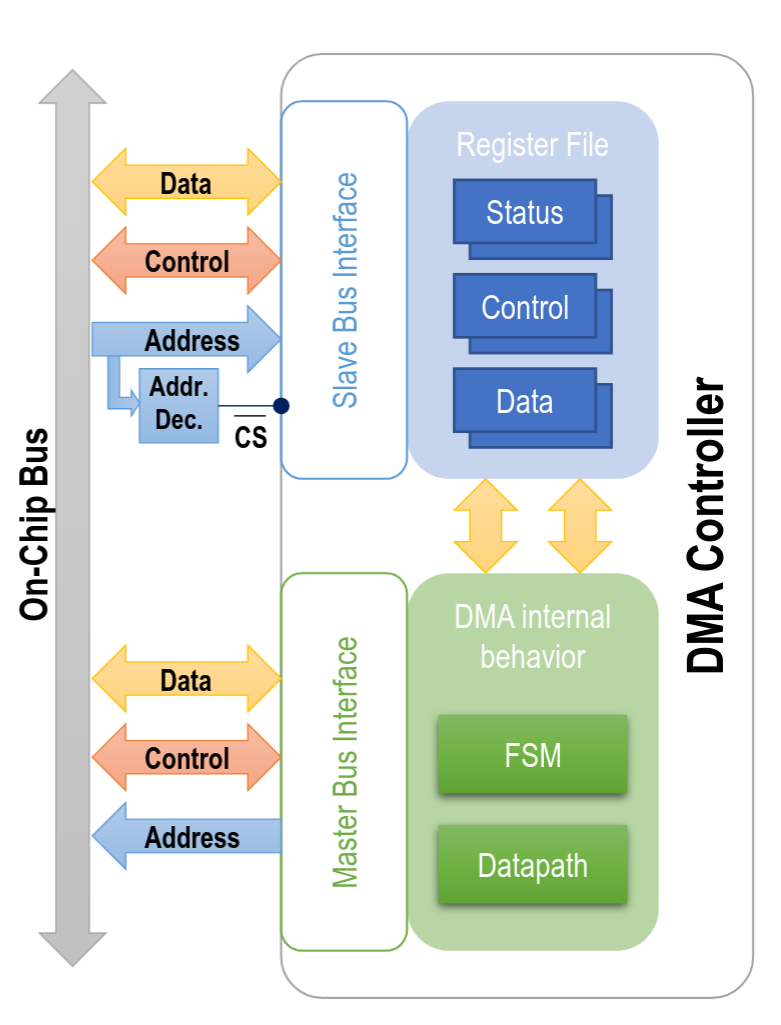
\includegraphics[scale=0.24]{../figures/dma.png}
\end{center}

As we can see, a DMA Controller has 2 interfaces:
\begin{itemize}
\item A \textbf{Slave} Bus Interface to access the peripheral registers, the same as a standard peripheral. This is used by the microprocessor core to:
\begin{itemize}
\item Configure the DMA controller
\item Check its status
\end{itemize}
\item A \textbf{Master} Bus Interface to generate bus transactions. It is used by the DMA controller internal behavior. It competes with other masters for the On-Chip Bus ownership (meaning we need arbitration on the On-Chip Bus). A DMA often has higher priority than a microprocessor core.
\end{itemize}

\subsubsection{External memory}

Similar to DMA (as in, it has 2 interfaces) is an \textbf{external memory controller}.

\begin{center}
	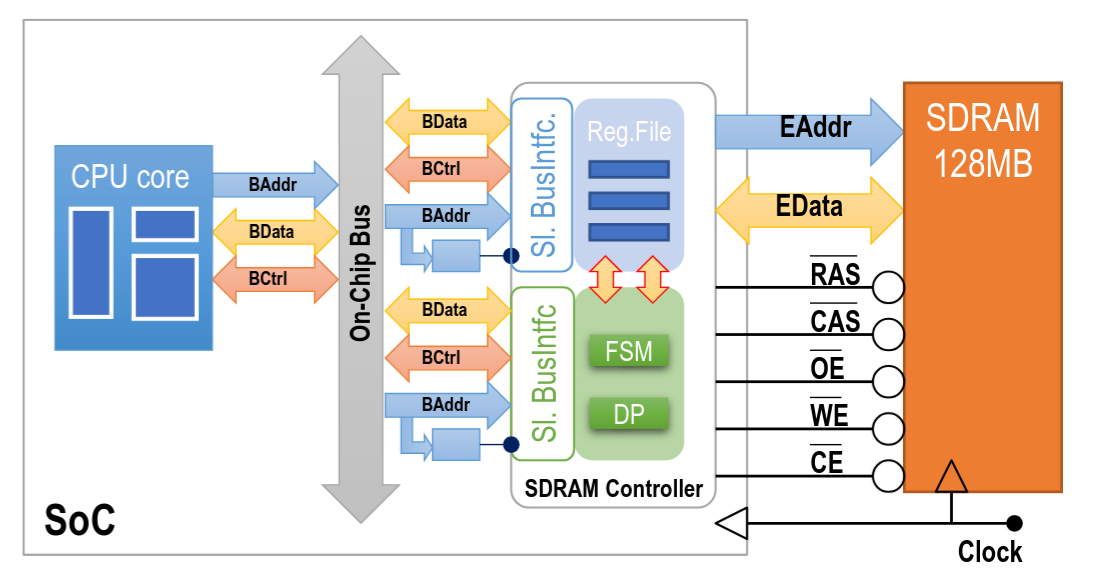
\includegraphics[scale=0.26]{../figures/ext_mem.png}
\end{center}

An External Memory Controller allows access to an external memory, such as \textit{asynchronous memories} (SRAM, E2PROM, Flash) or \texit{synchronous memories} (SDRAM, DDR).
It generates the proper access protocol, different depending on the memory kind.
For this reason, we need multiple controllers for different memory kinds.

Note that the controller responds to 2 distinct sets of addresses:
\begin{itemize}
\item The address range assigned to the peripheral registers (green);
\item The address range assigned to the external memory (blue).
\end{itemize}

\par\smallskip

To configure or read the state of the memory controller, the microprocessor core accesses the memory controller peripheral registers starting at the base address.
This is identical to a standard peripheral access, and allows access to control registers:
\begin{itemize}
\item Type of memory to be driven
\item Type of access (Page Mode, EDO, ...)
\item Number of banks
\item Word size
\item Burst size
\item Timing parameters (latency)
\end{itemize}

\par\smallskip

Then, o access the external memory the microprocessor core generates addresses assigned to the memory.
The transaction is initiated on the On-Chip Bus, and the same external memory controller detects the transactions.
It generates the proper external signals to access the memory, following memory protocol, and address translations.

It then reports on the On-Chip Bus the results: the microprocessor core only sees a standard On-Chip Bus transaction, possibly with some delay.

\end{document}
